\documentclass{standalone}
\usepackage{tikz}

\begin{document}

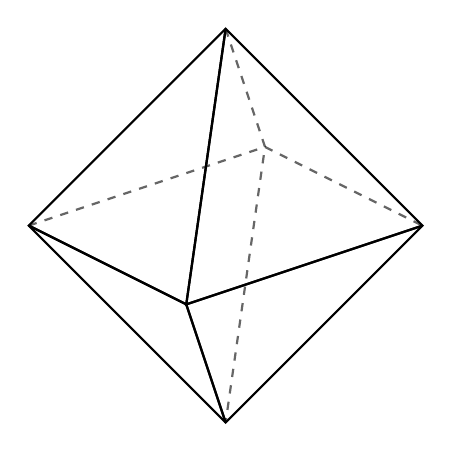
\begin{tikzpicture}[thick,scale=5]

\coordinate (A1) at (0,0);
\coordinate (A2) at (0.6,0.2);
\coordinate (A3) at (1,0);
\coordinate (A4) at (0.4,-0.2);
\coordinate (B1) at (0.5,0.5);
\coordinate (B2) at (0.5,-0.5);

\begin{scope}[thick,dashed,,opacity=0.6]
\draw (A1) -- (A2) -- (A3);
\draw (B1) -- (A2) -- (B2);
\end{scope}
\draw[solid] (A1) -- (A4) -- (B1);
\draw[solid] (A1) -- (A4) -- (B2);
\draw[solid] (A3) -- (A4) -- (B1);
\draw[solid] (A3) -- (A4) -- (B2);
\draw[solid] (B1) -- (A1) -- (B2) -- (A3) --cycle;

\end{tikzpicture}


\end{document}

% 正八面体

% convert -density 400 正八面体.pdf 正八面体.png